% =============================================================================
% paper.tex -- IEEE conference-format skeleton for the PMVC-WNM term paper.
%
% WHAT THIS IS: every table, figure, and bibliography entry is real and
% generated from the actual experiment results (see tables_generated.tex,
% built by ../build_latex_tables.py from results/*.csv). Every section of
% PROSE is left as a directive comment (%) telling you exactly what content
% and which numbers/citations go there -- per your course's Generative-AI
% policy, the sentences must be written by the team, not by an AI tool.
%
% If your course provided a specific IEEE template file/Overleaf link
% (the guidelines mention one), swap \documentclass[conference]{IEEEtran}
% for that exact template -- this uses the standard IEEEtran conference
% class as the closest general-purpose equivalent, since I don't have
% your course's specific template file.
% =============================================================================
\documentclass[conference]{IEEEtran}
\IEEEoverridecommandlockouts

\usepackage{amsmath,amssymb,amsfonts}
\usepackage{graphicx}
\usepackage{booktabs}
\usepackage{float}
\usepackage[numbers]{natbib}
\bibliographystyle{IEEEtranN}
\usepackage{hyperref}

\begin{document}

\title{% TODO: your final title, 10--15 words. Suggestions in the content
       % scaffold: e.g. "Two Views, One Bottleneck: An Empirical Study of
       % Co-Training for Code-Mixed Banglish Sentiment Analysis"
}

\author{
\IEEEauthorblockN{
% TODO: team member names
}
\IEEEauthorblockA{
% TODO: Department of CSE, Islamic University of Technology
}
}

\maketitle

\begin{abstract}
% TODO -- 150--250 words, write LAST, self-contained. Must cover in order:
%   1. Problem + significance: Banglish orthographic variation, sentiment
%      classification under limited labeled data.
%   2. Approach: two-view co-training (View A orthographic char n-gram TF-IDF
%      + View B phonetic-encoded TF-IDF) + weakly supervised noise model
%      (WNM), on an 11,788-row 3-class merged dataset.
%   3. Key results (pick 3-4, see Table \ref{tab:main-results} and the
%      Results section numbers below):
%      - reproduced the deployed pipeline within 0.003 macro-F1 of its own
%        logged run
%      - two-view ensembling alone gains ~+0.015 macro-F1 over baseline;
%        the co-training loop itself adds only ~+0.01 more
%      - exhaustive comparison of 21 classifiers found a better classifier
%        (Table \ref{tab:classifier-comparison}/\ref{tab:zoo-top5-viewA})
%      - the agreement gate's purity advantage inverts over iterations
%        (Figure \ref{fig:purity-trajectory})
%   4. Conclusion: PMVC-WNM does not significantly outperform standard
%      co-training on this data (inside seed noise) -- state this honestly;
%      frame the contribution as the diagnosis, not a claimed win.
\end{abstract}

\begin{IEEEkeywords}
% TODO: 4-6 keywords, e.g.: Banglish, code-mixed sentiment analysis,
% co-training, semi-supervised learning, classifier calibration
\end{IEEEkeywords}

% =============================================================================
\section{Introduction}
% See the separate Introduction LaTeX skeleton already provided in chat for
% the full paragraph-by-paragraph directive breakdown (hook / narrow / gap /
% contributions bullets / organization sentence). Paste that skeleton here
% once you've written the sentences, or ask for it again.
%
% Quick-reference numbers for the "narrow" paragraph:
%   - labeled seed = 600 rows; unlabeled pool ~8,830; full training pool
%     ~9,430 rows --> labeling rate ~6.4%.
%
% Contributions bullets should end with a \label{} you can \ref{} later if
% useful, and must be followed by one sentence on paper organization.

% =============================================================================
\section{Related Work}
% TODO 0.5-1.5 pages, >= 10 sources, organized THEMATICALLY with your own
% synthesizing prose (do not just list papers). Three clusters, with the
% verified citation keys already in references.bib:
%
% Cluster A -- Co-training / semi-supervised learning theory
%   \citep{blum1998combining} defines the core two-independent-views
%   assumption; \citep{vanengelen2020survey} frames declining view
%   independence over training as an open problem -- this is exactly what
%   your Results/Discussion measures directly (Figure
%   \ref{fig:purity-trajectory}).
%
% Cluster B -- Banglish / code-mixed sentiment analysis
%   \citep{alam2025bnsentmix} (BnSentMix, one of your three source
%   datasets) reports 69.8% transformer accuracy -- your framing: classical
%   models at 500-600 labels approach this without a GPU, not "beat
%   transformers." \citep{islam2023augmentation} and
%   \citep{sultana2024crosslingual} both use data augmentation as their
%   noise strategy; contrast with your WNM's LEARNED (not synthetic)
%   spelling-variant injection.
%
% Cluster C -- Feature engineering & classifier calibration
%   \citep{cavnar1994ngram} justifies char n-grams for noisy/varied text
%   (supports your Q2 char-vs-word finding, Table \ref{tab:ngram-budget}).
%   \citep{platt1999probabilistic} and \citep{niculescumizil2005predicting}
%   are your direct evidence base for the calibration discussion --- cite
%   Platt when explaining why full Platt scaling is slow; cite
%   Niculescu-Mizil & Caruana when discussing why an uncalibrated
%   margin-to-probability mapping is a poor confidence estimate (Table
%   \ref{tab:classifier-comparison}).
%
% VERIFY every citation against its primary source (Google Scholar / ACL
% Anthology / IEEE Xplore) before submitting -- some author lists in
% references.bib are abbreviated pending your verification.

% =============================================================================
\section{Dataset}
\label{sec:dataset}
% TODO. Content + exact numbers (all verified from common.py / results):
%   - 3 sources merged: BnSentMix (20,015 rows) \citep{alam2025bnsentmix},
%     b-and-b-80K (80,098 rows, native-Bengali column dropped)
%     \citep{kaggle_bandb80k}, EnBn-100K (100,000 rows).
%   - Merged + deduplicated (exact-text dedup) --> 186,138 rows.
%   - Balanced sample: 11,788 rows (Negative 3,889 / Neutral 4,000 /
%     Positive 3,899).
%   - Label unification table -- TODO: format as a \begin{table} with the
%     mapping (BnSentMix numeric 0/1/2,3,4 -> Positive/Negative/Neutral;
%     emotion words similarly mapped, see chat history for the full map).
%   - Split: 80/20 stratified train/test; 600-row stratified labeled seed
%     from the training pool; ~8,830-row unlabeled pool. 3 seeds (42, 7,
%     2024), every reported number averaged over these.
%   - Representative samples: pull 2-3 REAL rows yourself from the data
%     (do not fabricate examples) -- e.g. via
%     \texttt{build\_working\_set().head()} in \texttt{common.py}.
%   - Preprocessing WITH justification: lowercase, strip URLs, keep
%     Roman letters/digits, collapse 3+ repeated chars; justify as
%     normalizing emphatic typing without destroying word identity.
%   - Limitations (be honest, rubric wants this): "Neutral" folds two
%     distinct phenomena (BnSentMix's "mixed" + "surprise") into one
%     class -- reference the 0.6562 full-supervision ceiling (Table
%     \ref{tab:main-results}) as direct evidence this bounds achievable
%     performance regardless of model choice. The three sources differ in
%     genre (comments vs. reviews), a possible domain-shift risk.

% =============================================================================
\section{Methodology}
\label{sec:methodology}
% TODO 1-2.5 pages. Formal problem definition, then per-component
% description with hyperparameters AND justification (rubric requirement):
%
%   Problem: given Banglish text x, predict y in {Positive, Negative,
%   Neutral}. Views phi_A(x) (char n-gram TF-IDF) and phi_B(x) (phonetic
%   TF-IDF) trained independently; co-training alternates f_A, f_B on a
%   seed set L and a growing pseudo-labeled subset of pool U.
%
%   View A: char\_wb analyzer, n-gram (3,4), max\_features=5000.
%   Classifier: LinearSVC + softmax(decision margins, T=2.0) for
%   confidence. Justify via \citep{platt1999probabilistic}: full Platt
%   scaling measured ~50x slower (1.44s vs.\ 0.02s, Table
%   \ref{tab:classifier-comparison}).
%
%   View B: word-level TF-IDF (1,2) over a Soundex-style phonetic
%   encoding (briefly define the digraph-first greedy encoding rule).
%   Classifier: Logistic Regression (C=5, max\_iter=2000).
%
%   Co-training loop: N\_ITER=12, STEP=450 pseudo-labels/iteration,
%   CONF\_THRESHOLD=0.55. Two selection rules compared (Table
%   \ref{tab:gate-comparison}): standard (View A confidence alone) vs.\
%   PMVC-WNM (agreement gate: both views agree AND both exceed threshold,
%   ranked by conf\_A * conf\_B).
%
%   WNM: class-confusion transition matrix from View A/B disagreements;
%   diagonal used as per-class reliability weight; ~35% token-level
%   phonetic-variant corruption (bh<->v, sh<->s, ch<->c, kh<->k, gh<->g,
%   th<->t, ph<->f, jh<->j, o<->u, i<->e) re-injected into View A's
%   training data at half sample-weight.
%
%   Metrics (DEFINE + JUSTIFY each, not just name):
%     - Macro-F1 (primary): unweighted mean of per-class F1.
%     - Accuracy: reported alongside for interpretability.
%     - Brier score (one-vs-rest, averaged): used specifically in Table
%       \ref{tab:classifier-comparison} to quantify calibration
%       independent of accuracy -- justify via
%       \citep{niculescumizil2005predicting}.
%
%   Baselines (Table \ref{tab:main-results}): single-view SVM; standard
%   co-training (no WNM); full-supervision upper bound.
%
%   Exhaustive classifier comparison protocol: 21 classifiers across 7 ML
%   families, each evaluated via 5-fold stratified CV on the 600-row seed
%   AND held-out test performance over 3 seeds -- describe why both
%   (Figure \ref{fig:cv-vs-holdout} exposes overfitting risk that holdout
%   alone would hide).
%
%   Reproducibility: state the 3-seed protocol, and that all code and
%   exact hyperparameters are in the repository \citep{pmvcwnm_repo}.

% =============================================================================
\section{Results}
\label{sec:results}
% TODO. Report OBJECTIVELY -- include the PMVC-WNM vs.\ standard result
% even though it's not flattering (+0.0013, inside seed std ~0.01).
%
% Main results table:
% AUTO-GENERATED by build_latex_tables.py -- do not hand-edit.
% Re-run the script if results/*.csv change.

\begin{table}[t]
\centering
\caption{Main results: macro-F1 on the held-out test set, mean over 3 seeds (42, 7, 2024).}
\label{tab:main-results}
\begin{tabular}{lc}
\toprule
\textbf{Model} & \textbf{Macro-F1} \\
\midrule
Single-view SVM (baseline) & 0.5534 \\
Standard co-training (no WNM) & 0.5767 \\
PMVC-WNM (deployed) & 0.5794 \\
Best exhaustive candidate, View A (\texttt{ridge\_calibrated}) & 0.5652 \\
Best exhaustive candidate, View B (\texttt{ridge\_calibrated}) & 0.5542 \\
Full-supervision ceiling ($\sim$9{,}430 labels) & 0.6562 \\
\bottomrule
\end{tabular}
\end{table}


\begin{table}[t]
\centering
\caption{View A / View B classifier comparison (mean over 3 seeds). Lower Brier score indicates better-calibrated confidence estimates.}
\label{tab:classifier-comparison}
\begin{tabular}{llrrr}
\toprule
\textbf{View} & \textbf{Classifier} & \textbf{Macro-F1} & \textbf{Brier} & \textbf{Fit (s)} \\
\midrule
A & \texttt{svm\_platt} & 0.5624 & 0.1807 & 1.435 \\
A & \texttt{logreg} & 0.5613 & 0.1802 & 0.729 \\
A & \texttt{svm\_calibrated} & 0.5596 & 0.1813 & 0.120 \\
A & \texttt{svm\_softmax} & 0.5534 & 0.1960 & 0.018 \\
B & \texttt{logreg} & 0.5522 & 0.1845 & 1.314 \\
B & \texttt{svm\_softmax} & 0.5488 & 0.2002 & 0.007 \\
B & \texttt{complement\_nb} & 0.5340 & 0.1952 & 0.005 \\
B & \texttt{random\_forest} & 0.5245 & 0.1907 & 1.492 \\
\bottomrule
\end{tabular}
\end{table}


\begin{table}[t]
\centering
\caption{Feature n-gram range comparison at the deployed 5{,}000-feature budget (mean over 3 seeds).}
\label{tab:ngram-budget}
\begin{tabular}{llr}
\toprule
\textbf{View} & \textbf{Config} & \textbf{Macro-F1} \\
\midrule
A & char(2,3) & 0.5611 \\
A & char(3,4) [deployed] & 0.5534 \\
B & word(1,1) & 0.5575 \\
B & word(1,2) [deployed] & 0.5522 \\
\bottomrule
\end{tabular}
\end{table}


\begin{table}[t]
\centering
\caption{Pseudo-label gate comparison, confidence threshold fixed at 0.55 (mean $\pm$ std over 3 seeds).}
\label{tab:gate-comparison}
\begin{tabular}{lrrr}
\toprule
\textbf{Gate} & \textbf{Macro-F1} & \textbf{Pseudo-labels} & \textbf{Purity} \\
\midrule
agreement\_and\_confident (pmvc\_wnm) & 0.5794 $\pm$ 0.0094 & 7191 & 0.859 \\
view\_a\_only (standard) & 0.5767 $\pm$ 0.0101 & 5783 & 0.881 \\
agreement\_or\_one\_very\_confident & 0.5739 $\pm$ 0.0058 & 21827 & 0.757 \\
agreement\_no\_threshold & 0.5701 $\pm$ 0.0077 & 35100 & 0.709 \\
or\_union & 0.5701 $\pm$ 0.0077 & 35100 & 0.673 \\
\bottomrule
\end{tabular}
\end{table}


\begin{table}[t]
\centering
\caption{Cumulative single-view (View A) improvement ladder, each row adds one change on top of the previous (mean over 3 seeds).}
\label{tab:improvement-ladder}
\begin{tabular}{lr}
\toprule
\textbf{Configuration} & \textbf{Macro-F1} \\
\midrule
0. baseline (svm\_softmax, char(3,4), 5k feat) & 0.5534 $\pm$ 0.0120 \\
1. max\_features=50000 & 0.5729 $\pm$ 0.0036 \\
2. + min\_df=2 & 0.5733 $\pm$ 0.0016 \\
3. + class\_weight=balanced & 0.5741 $\pm$ 0.0024 \\
4. + C tuned (C=0.3) & 0.5751 $\pm$ 0.0028 \\
5. + word(1,2) UNION char(3,5) [50k total] & 0.5830 $\pm$ 0.0019 \\
6. + CalibratedClassifierCV(LinearSVC) & 0.5849 $\pm$ 0.0032 \\
\bottomrule
\end{tabular}
\end{table}


\begin{table}[t]
\centering
\caption{Top 5 of 21 candidates tested, View A (mean over 3 seeds).}
\label{tab:zoo-top5-viewA}
\begin{tabular}{llrrr}
\toprule
\textbf{Model} & \textbf{Family} & \textbf{Holdout F1} & \textbf{CV F1} & \textbf{Fit (s)} \\
\midrule
\texttt{ridge\_calibrated} & linear & 0.5652 $\pm$ 0.0064 & 0.6688 & 0.08 \\
\texttt{logreg} & linear & 0.5613 $\pm$ 0.0089 & 0.6599 & 1.40 \\
\texttt{bagging\_linsvc} & tree\_ensemble & 0.5601 $\pm$ 0.0013 & 0.6631 & 0.08 \\
\texttt{linsvc\_calibrated} & linear & 0.5596 $\pm$ 0.0065 & 0.6642 & 0.08 \\
\texttt{knn\_k15} & instance\_based & 0.5541 $\pm$ 0.0069 & 0.6199 & 0.00 \\
\bottomrule
\end{tabular}
\end{table}


\begin{table}[t]
\centering
\caption{Top 5 of 21 candidates tested, View B (mean over 3 seeds).}
\label{tab:zoo-top5-viewB}
\begin{tabular}{llrrr}
\toprule
\textbf{Model} & \textbf{Family} & \textbf{Holdout F1} & \textbf{CV F1} & \textbf{Fit (s)} \\
\midrule
\texttt{ridge\_calibrated} & linear & 0.5542 $\pm$ 0.0076 & 0.6446 & 0.06 \\
\texttt{logreg} & linear & 0.5522 $\pm$ 0.0076 & 0.6381 & 0.58 \\
\texttt{linsvc\_calibrated} & linear & 0.5519 $\pm$ 0.0074 & 0.6420 & 0.05 \\
\texttt{linsvc\_softmax} & linear & 0.5488 $\pm$ 0.0065 & 0.6359 & 0.01 \\
\texttt{bagging\_linsvc} & tree\_ensemble & 0.5471 $\pm$ 0.0065 & 0.6377 & 0.05 \\
\bottomrule
\end{tabular}
\end{table}


\begin{table}[t]
\centering
\caption{Label-budget sensitivity: team's deployed model vs.\ best-found model (mean over 3 seeds).}
\label{tab:budget-sensitivity}
\begin{tabular}{lrrrr}
\toprule
\textbf{Labeled seed} & \textbf{Team A} & \textbf{Best A} & \textbf{Team B} & \textbf{Best B} \\
\midrule
300 & 0.5376 & 0.5466 & 0.5176 & 0.5126 \\
600 & 0.5534 & 0.5652 & 0.5522 & 0.5542 \\
900 & 0.5669 & 0.5813 & 0.5701 & 0.5729 \\
1200 & 0.5908 & 0.6017 & 0.5830 & 0.5848 \\
\bottomrule
\end{tabular}
\end{table}


\begin{table}[t]
\centering
\caption{Spelling-noise robustness: macro-F1 under injected phonetic-variant corruption (mean over 3 seeds).}
\label{tab:noise-robustness}
\begin{tabular}{lrrrr}
\toprule
\textbf{Noise rate} & \textbf{Team A} & \textbf{Best A} & \textbf{Team B} & \textbf{Best B} \\
\midrule
0\% & 0.5534 & 0.5652 & 0.5522 & 0.5542 \\
20\% & 0.5486 & 0.5614 & 0.5516 & 0.5535 \\
35\% & 0.5444 & 0.5554 & 0.5524 & 0.5548 \\
\bottomrule
\end{tabular}
\end{table}

% (all 9 tables from build_latex_tables.py are inserted above, in this
%  order: main results, Q1 classifier comparison, Q2 n-gram budget, Q3
%  gate comparison, Q4 improvement ladder, exhaustive top-5 View A, top-5
%  View B, budget sensitivity, noise robustness. Move/reorder \input
%  blocks individually if you want a different order -- open
%  tables_generated.tex and split by \begin{table} if so.)
%
% Figures to place near their relevant discussion (all in figures/):
\begin{figure}[t]
\centering
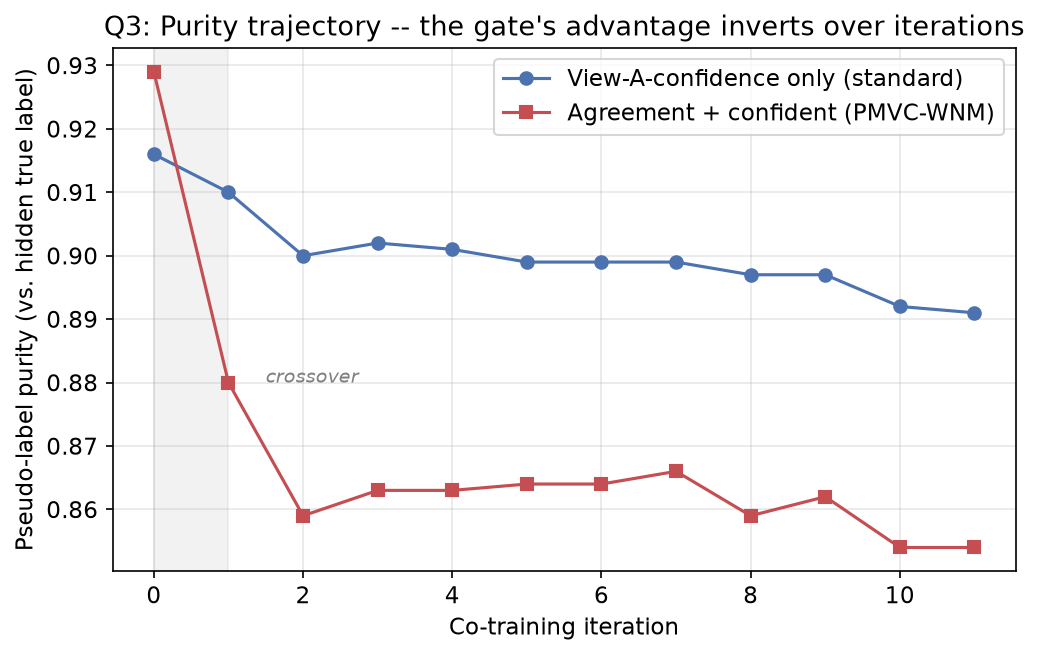
\includegraphics[width=\linewidth]{figures/fig2_purity_trajectory.png}
\caption{Pseudo-label purity by co-training iteration, seed 42. The
agreement gate's purity advantage appears only at iteration 0 and inverts
by the final iteration.}
\label{fig:purity-trajectory}
\end{figure}

\begin{figure}[t]
\centering
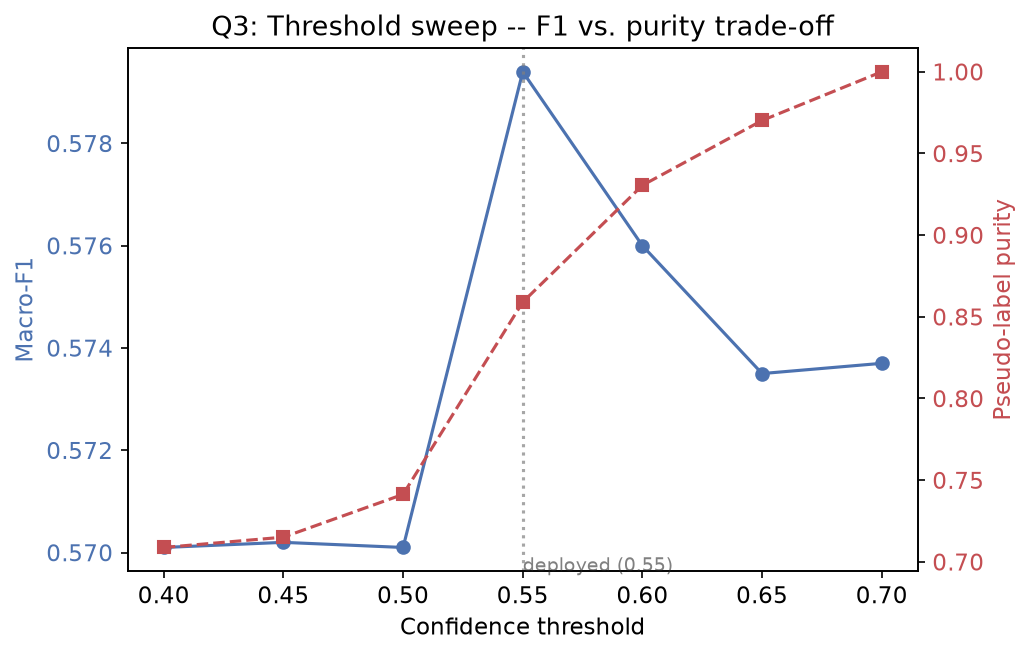
\includegraphics[width=\linewidth]{figures/fig3_threshold_sweep.png}
\caption{Macro-F1 (left axis) and pseudo-label purity (right axis) vs.\
confidence threshold on the deployed agreement gate.}
\label{fig:threshold-sweep}
\end{figure}

\begin{figure}[t]
\centering
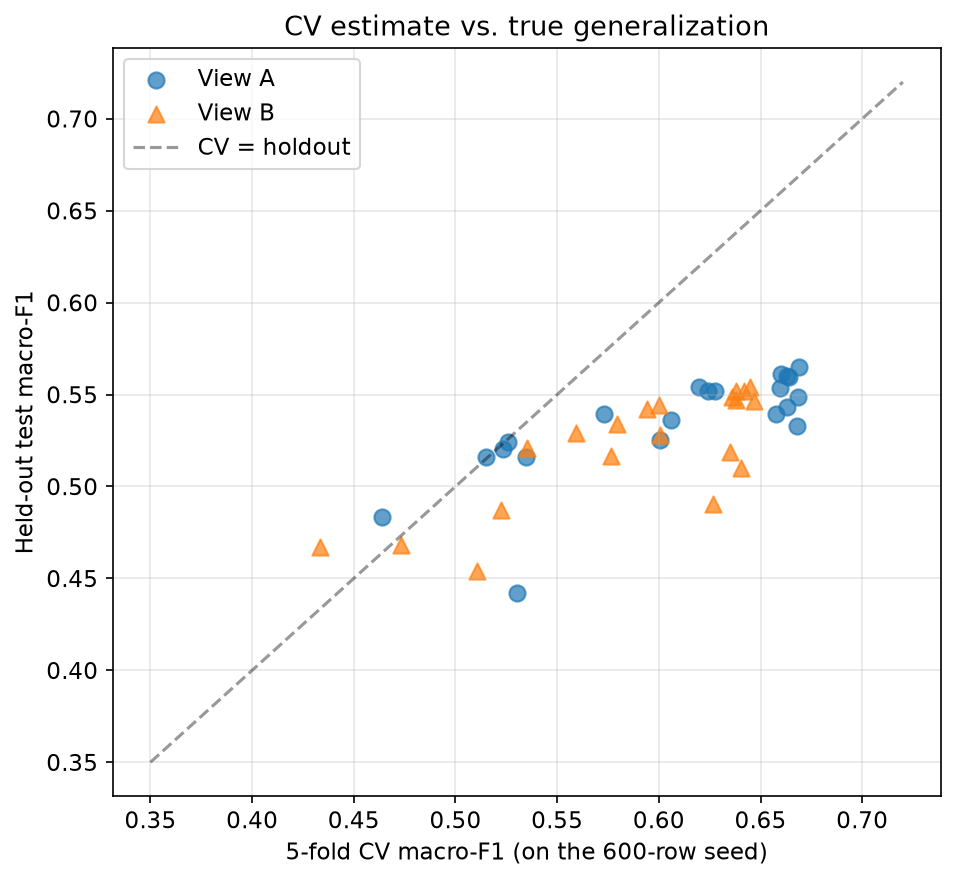
\includegraphics[width=\linewidth]{figures/fig6_cv_vs_holdout.png}
\caption{Every candidate's 5-fold CV estimate vs.\ its held-out test
score. Points below the diagonal generalize worse than their CV estimate
suggested.}
\label{fig:cv-vs-holdout}
\end{figure}

\begin{figure}[t]
\centering
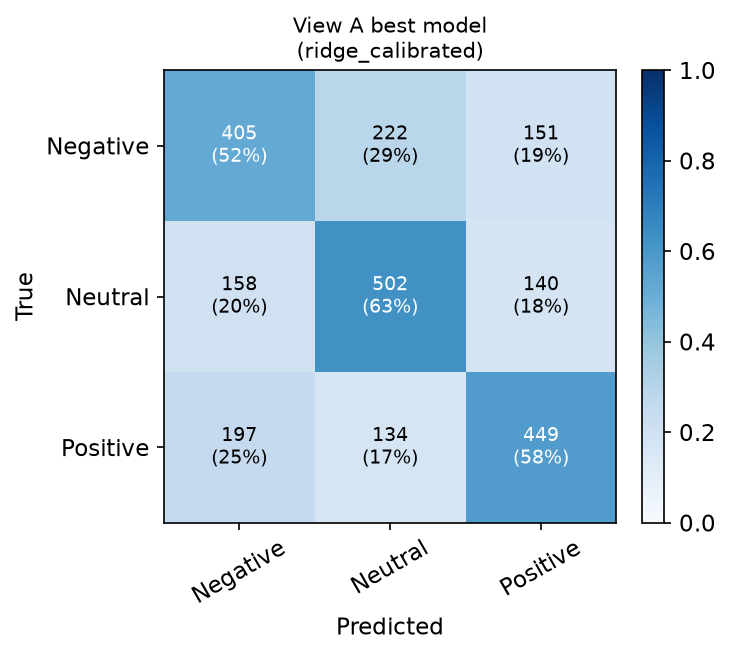
\includegraphics[width=0.48\linewidth]{figures/fig9_confusion_viewA.png}
\hfill
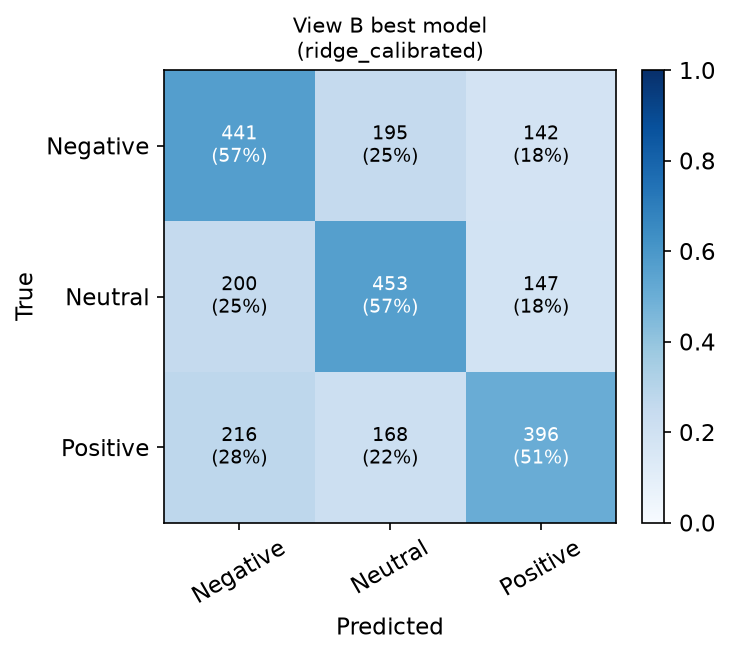
\includegraphics[width=0.48\linewidth]{figures/fig9_confusion_viewB.png}
\caption{Row-normalized confusion matrices, best model per view, seed 42.}
\label{fig:confusion}
\end{figure}

% Optional additional figures available in figures/ if you want them:
%   fig1_classifier_comparison.png, fig4_improvement_ladder.png,
%   fig5_exhaustive_zoo_viewA.png, fig5_exhaustive_zoo_viewB.png,
%   fig7_budget_sensitivity.png, fig8_noise_robustness.png
% Six-figure IEEE conference papers get long fast -- pick the ones that
% carry the most weight for YOUR narrative rather than including all 11.

% =============================================================================
\section{Discussion}
\label{sec:discussion}
% TODO. Interpret, don't restate. Talking points (write your own analysis):
%   - What the results mean for the research question: co-training helps
%     mostly through the ENSEMBLE mechanism, not iterative pseudo-labeling
%     -- reframe what "co-training" actually buys here vs.\ the original
%     proposal's framing.
%   - Why some models outperform others: tie to feature-space geometry --
%     linear models suit sparse high-dim TF-IDF; every tree/ensemble/
%     boosting candidate underperformed every linear candidate (Tables
%     \ref{tab:zoo-top5-viewA}, \ref{tab:zoo-top5-viewB}). Calibration
%     quality (not just separability) determines whether the 0.55
%     threshold behaves as intended -- tie back to
%     \citep{platt1999probabilistic,niculescumizil2005predicting}.
%   - Hardest cases: read your actual confusion matrices (Figure
%     \ref{fig:confusion}) and name the specific class pattern -- likely
%     "Neutral" absorbing two distinct phenomena (Section
%     \ref{sec:dataset}'s limitation).
%   - Consistency with literature: linear-beats-tree-on-sparse-text is
%     consistent with established text-classification results
%     \citep{cavnar1994ngram}; frame this as confirmation. The
%     purity-inversion finding (Figure \ref{fig:purity-trajectory}) is
%     the part genuinely novel to this paper -- say so explicitly.
%   - What you'd do differently: multi-seed CV (currently one seed only,
%     state this as a limitation); a 4-class scheme instead of folding
%     "mixed" into Neutral; testing whether purity inversion generalizes
%     beyond this gate design.

% =============================================================================
\section{Conclusion}
% TODO 1-2 paragraphs, NO new information, NO reflective language
% ("valuable learning experience" etc. -- rubric explicitly forbids this).
% Structure: (a) restate 2-3 strongest findings in one sentence each
% (ensemble-vs-iteration decomposition; purity-inversion; exhaustive-
% comparison result); (b) state plainly what was learned about which of
% the original design choices were justified vs.\ not (Q1-Q4); (c) point
% to future work already listed in Discussion.

% =============================================================================
% AI Usage Statement -- MANDATORY per course guidelines Section 4.2.
% Write this yourself, accurately. It must honestly state (see full
% content-scaffold doc / chat for the detailed breakdown):
%   - AI was used to write/debug the Python experiment scripts (permitted).
%   - AI was used to understand co-training/calibration concepts and to
%     locate/verify literature references (permitted) -- note you must
%     NOT cite an AI tool as a source anywhere in the paper.
%   - AI produced a content scaffold/outline and this LaTeX skeleton
%     (tables/figures/structure only) used as reference while drafting;
%     state clearly that the prose was written by the team.
%   - If AI proofread any drafted section, name that specifically.
% \section*{AI Usage Statement}
% TODO

% =============================================================================
\bibliography{references}

\end{document}
